\chapter*{Anexos}

\begin{figure}
\begin{center}
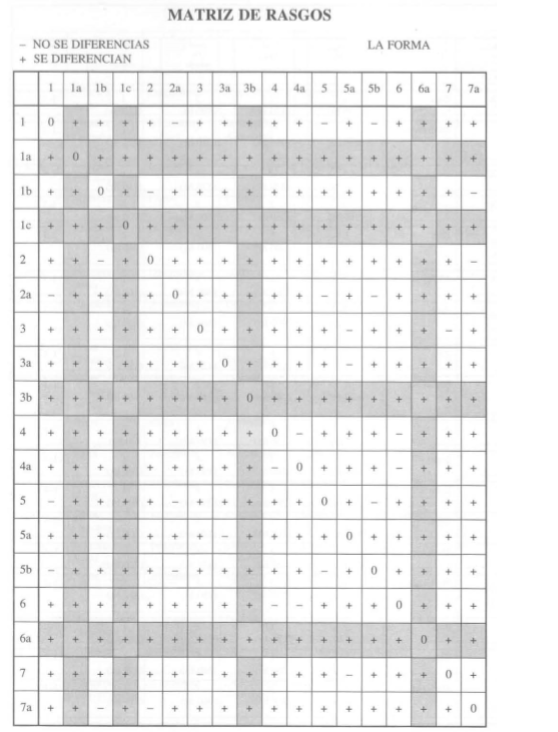
\includegraphics[width= 0.7\columnwidth]{Graphics/rasgos_forma}
\caption{Diferenciaci\'on en cuanto a la \emph{forma} de la curva mel\'odica. Tomado de \cite[p.220]{garcia1996aspectos2}.}
\label{rasgos_forma}
\end{center}
\end{figure}


\begin{figure}
\begin{center}
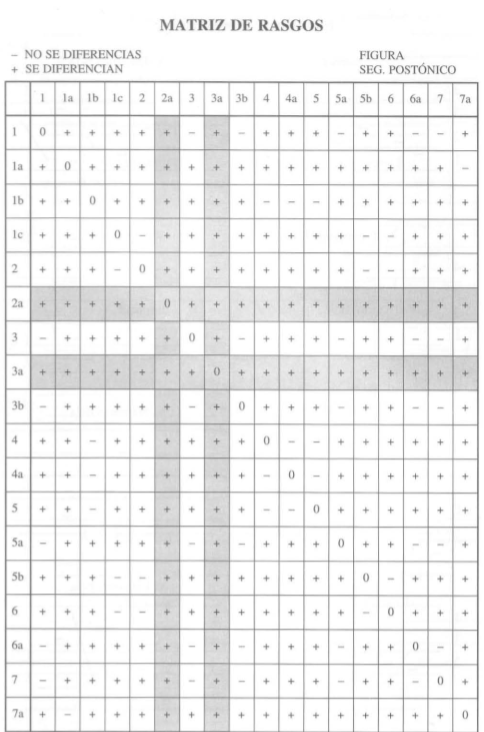
\includegraphics[width= 0.7\columnwidth]{Graphics/rasgos_figura}
\caption{Diferenciaci\'on en cuanto a la \emph{figura del segmento post\'onico}. Tomado de \cite[p.221]{garcia1996aspectos2}.}
\label{rasgos_figura}
\end{center}
\end{figure}


\begin{figure}
\begin{center}
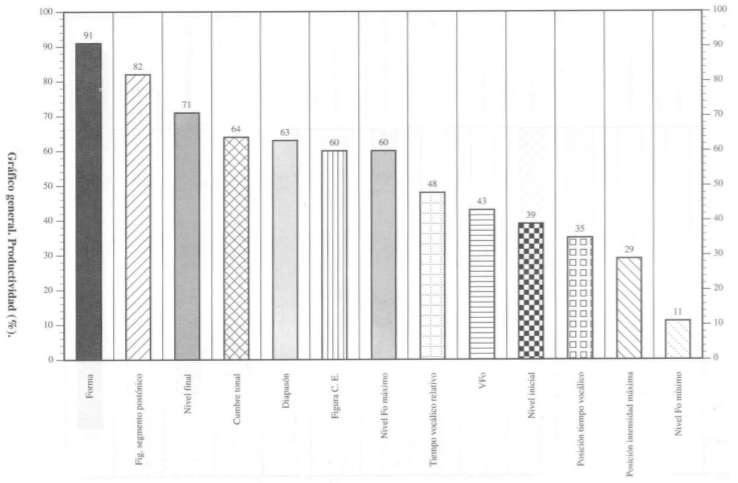
\includegraphics[width= 0.7\columnwidth]{Graphics/productividad}
\caption{Productividad de los rasgos distintivos en la investigaci\'on de Garc\'ia River\'on. Tomado de \cite[p.233]{garcia1996aspectos2}.}
\label{productividad}
\end{center}
\end{figure}

\begin{figure}
\begin{center}
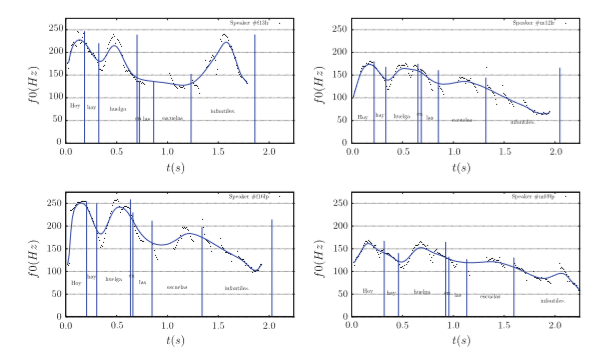
\includegraphics[width= 1\columnwidth]{Graphics/diferencialocutor}
\caption{Contorno mel\'odico de la frase ``Hoy hay huelga en las escuelas infantiles'' pronunciado por 4 individuos diferentes. Tomado de \cite[p.966]{garrido2013glissando}.}
\label{diferencialocutor}
\end{center}
\end{figure}


\begin{figure}
\begin{center}
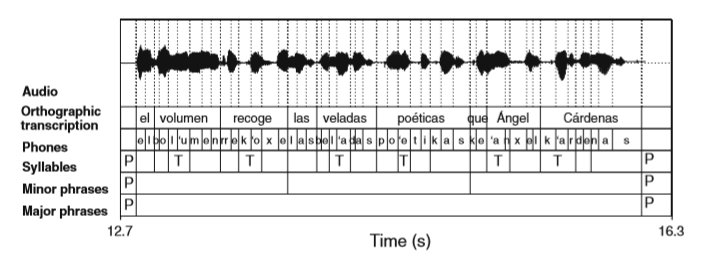
\includegraphics[width= 1\columnwidth]{Graphics/textgrid}
\caption{TextGrid de Praat de ejemplo. Tomado de \cite[p.962]{garrido2013glissando}.}
\label{textgrid}
\end{center}
\end{figure}


\begin{figure}
\begin{center}
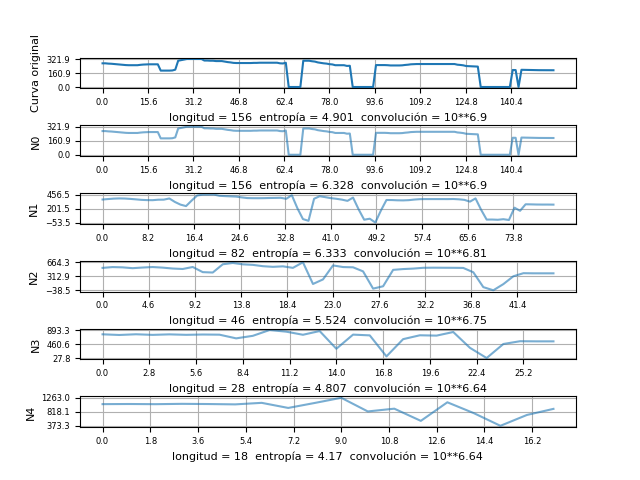
\includegraphics[width= 1\columnwidth]{Graphics/reconstruccion}
\caption{Reconstrucci\'on de la curva mel\'odica con los coeficientes de aproximaci\'on y de detalle de los niveles 0 al 4 en la DWT con Daubechies. Se muestra la entrop\'ia de la curva reconstruida en cada nivel, la longitud de la misma y su convoluci\'on con la curva original.}
\label{reconstruccion}
\end{center}
\end{figure}


\begin{figure}
\begin{center}
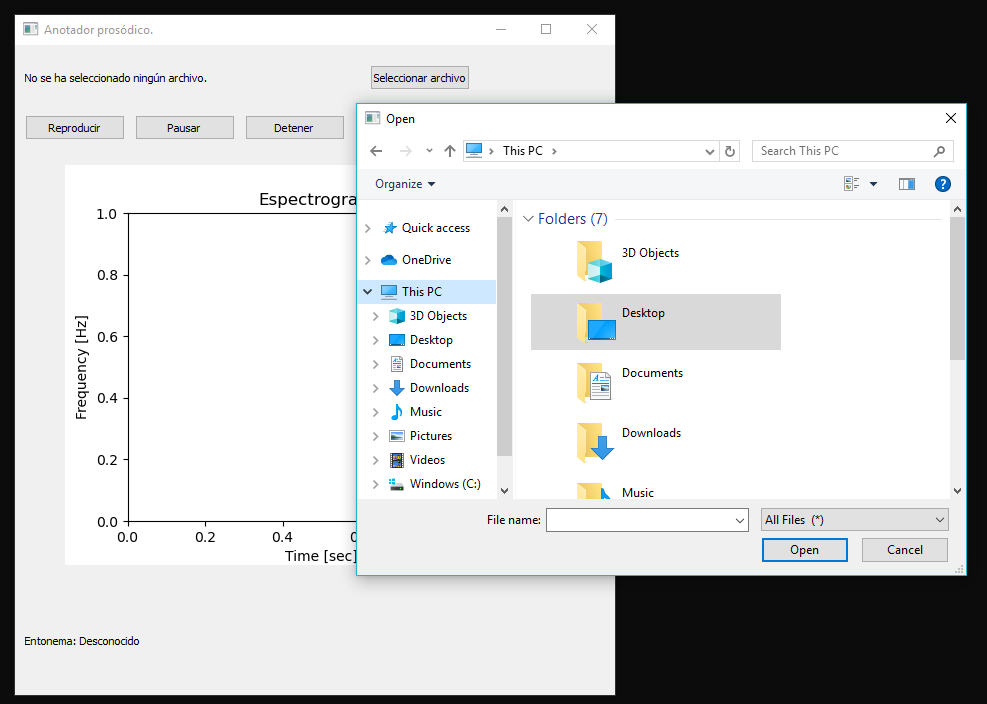
\includegraphics[width= 1\columnwidth]{Graphics/software}
\caption{Interfaz gr\'afica del software desarrollado. Su uso es simple: al presionar el bot\'on \emph{Seleccionar archivo} aparece un cuadro de di\'alogo para explorar y seleccionar el .wav que se desea analizar. Autom\'aticamente se grafica el espectrograma asociado y se muestra en la etiqueta inferior izquierda el entonema que se predice para el archivo seleccionado. Los botones \emph{Reproducir}, \emph{Pausar} y \emph{Detener} son para manipular el audio que est\'e seleccionado, cuyo nombre se muestra en la etiqueta superior izquierda. Un resultado de ejemplo se observa en la Figura \ref{software2}.}
\label{software}
\end{center}
\end{figure}

\begin{figure}
\begin{center}
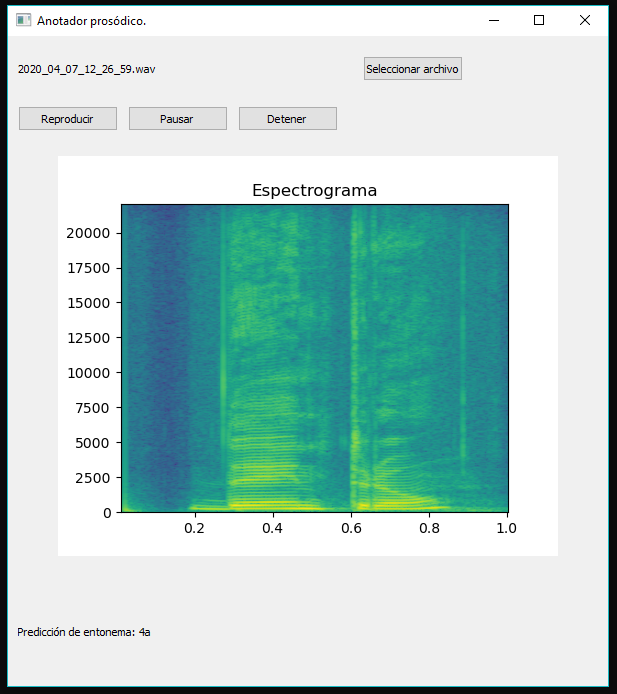
\includegraphics[width= 1\columnwidth]{Graphics/software2}
\caption{Interfaz gr\'afica del software desarrollado. Se muestra el espectrograma para el audio 2020\_04\_07\_12\_26\_59.wav y se predice por el algoritmo de aprendizaje que presenta el entonema \emph{4a}.}
\label{software2}
\end{center}
\end{figure}